\documentclass[conference]{IEEEtran}
%\IEEEoverridecommandlockouts
% The preceding line is only needed to identify funding in the first footnote. If that is unneeded, please comment it out.
% Template version as of 6/27/2024

\usepackage{cite}
\usepackage[ngerman]{babel}
\usepackage{amsmath,amssymb,amsfonts}
\usepackage{algorithmic}
\usepackage{graphicx}
\usepackage{textcomp}
\usepackage{xcolor}
%\usepackage{todonotes}
\newcommand{\todo}[1]{\textcolor{red}{TODO: #1}}
\def\BibTeX{{\rm B\kern-.05em{\sc i\kern-.025em b}\kern-.08em
    T\kern-.1667em\lower.7ex\hbox{E}\kern-.125emX}}
\begin{document}

\title{FPGAs in DBMS
}

\author{\IEEEauthorblockN{1\textsuperscript{st} Felix Grenzing}
    \IEEEauthorblockA{\textit{Universität Hamburg} \\
        Hamburg, Deutschland\\
        felix.grenzing@studium.uni-hamburg.de}
}

\maketitle

\begin{abstract}
    Abstract here.
\end{abstract}

\begin{IEEEkeywords}
    FPGAs, DBMS, Hardware Acceleration
\end{IEEEkeywords}

\section{Einführung}


\section{Begriffe}
In \cite{li_bitweaving_2013} und \cite{lisa_column_2018} werden verschidene Begriffe verwendet, die Erklärung bedürfen.


\subsection{FPGAs}


\subsection{Einsatzmöglichkeiten}


\begin{figure}[htbp]
    \centering
    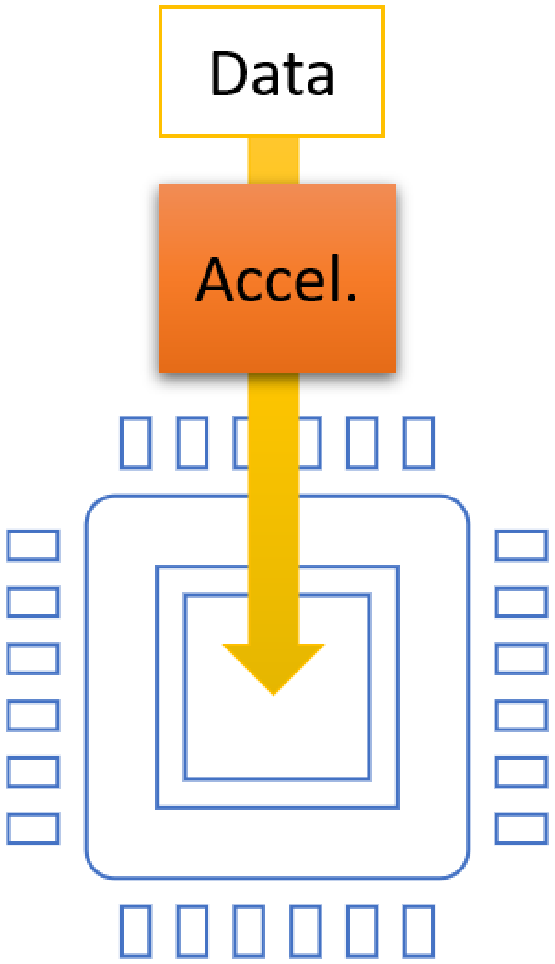
\includegraphics[width=0.1\textwidth]{imgs/InDatapath.png}
    \caption{In Datapath Architektur}
    \label{fig:indatapath}
\end{figure}

\begin{figure}[htbp]
    \centering
    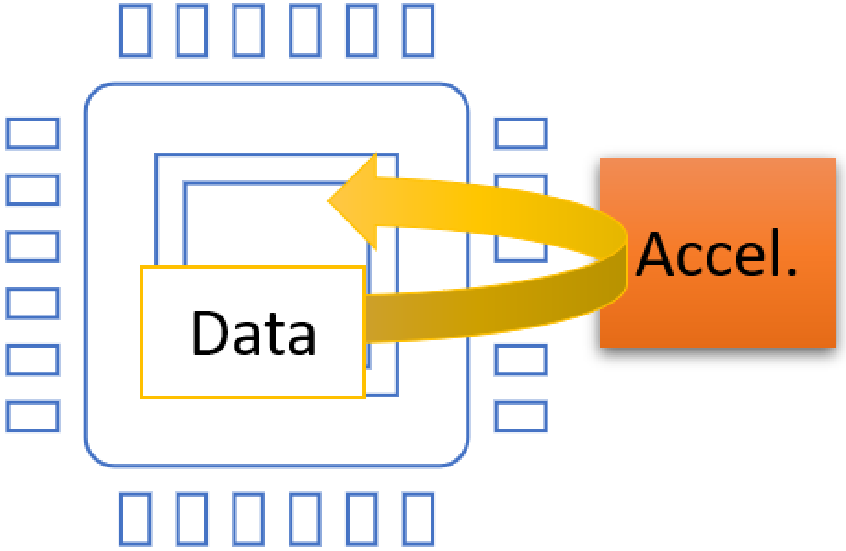
\includegraphics[width=0.15\textwidth]{imgs/OnTheSide.png}
    \caption{On The Side Architektur}
    \label{fig:ontheside}
\end{figure}


\begin{figure}[htbp]
    \centering
    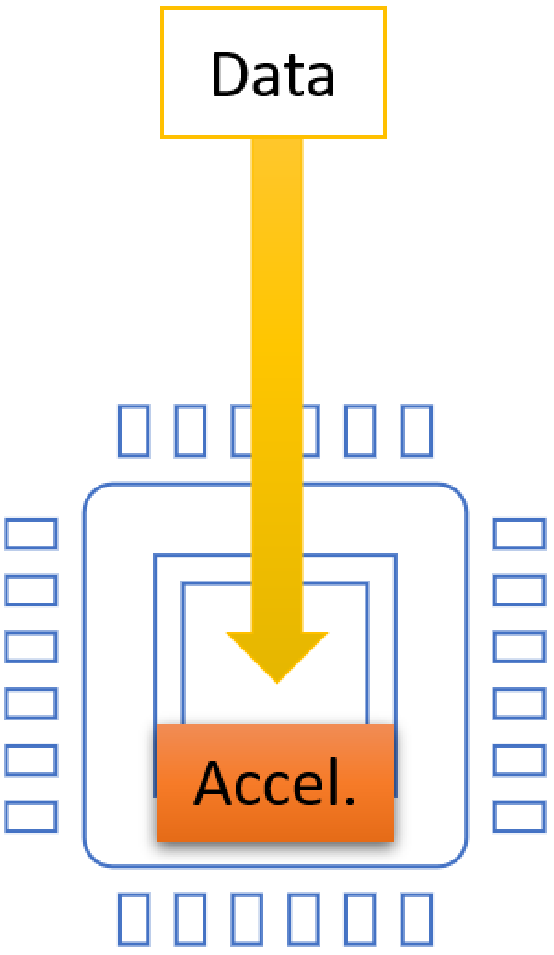
\includegraphics[width=0.1\textwidth]{imgs/Coprocessor.png}
    \caption{Koprozessor Architektur}
    \label{fig:coprocessor}
\end{figure}

\subsection{Pipelining und Datenparallelität}
Zwei wichtige Arten der Parallelität sind die Pipelineparallelität und die Datenparallelität. Pipelineparalleität beschreibt die Aufteilung der Befehlsabarbeitung
in mehrere Stufen, die parallel arbeiten. Jede Stufe bearbeitet dabei Teil des Befehls und gibt die Ergebnisse an die nächste Stufe weiter.
Ein Beispiel für eine Pipeline ist in Abbildung~\ref{fig:pipeline} zu sehen. Die Befehle werden in vier Stufen aufgeteilt. Bearbeitet die Fetch Stufe den ersten Befehl.
Sobald dies geschehen ist, wird der Befehl an die nächste Stufe weitergegeben. Die Fetch Stufe kann nun den nächsten Befehl bearbeiten. Die Befehle werden so stufenweise
durch die Pipeline geschoben.

Datenparallelität beschreibt die Aufteilung der Daten in mehrere Teile, die mit mehreren Bearbeitungseinheiten parallel verarbeitet werden. Beide Ansätze können die Performance
von Algorithmen verbessern, und können auch kombiniert werden um die Vorteile beider Ansätze zu nutzen. Um beide Ansätze zu kombinieren, könnten mehrere Pipelines entworfen werden,
die jeweils verschidene Datenbearbeiten.

\begin{figure}[htbp] % https://en.wikipedia.org/wiki/Instruction_pipelining#/media/File:Pipeline,_4_stage.svg
    \centering
    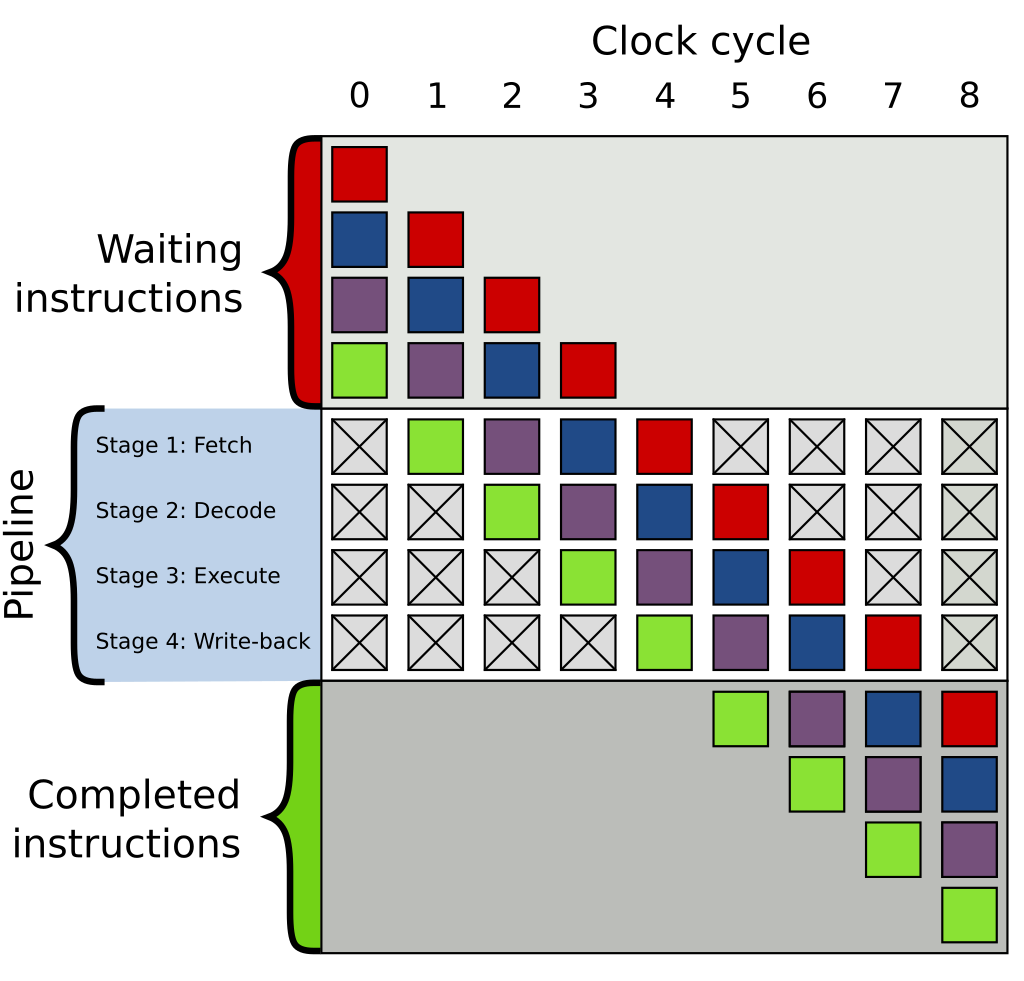
\includegraphics[width=0.25\textwidth]{imgs/pipeline.png}
    \caption{Prozessor Pipeline}
    \label{fig:pipeline}
\end{figure}


\subsection{Partial Reconfiguration}
Partial Reconfiguration (PR) ist ein Konzept, welches aktuelle FPGAs unterstützen. PR bietet die Möglichkeit, Teile des FPGAs zur Laufzeit zu verändern,
ohne das gesamte FPGA neu zu konfigurieren oder das FPGA offline nehmen zu müssen. Dies ermöglicht es, verschiedene Funktionen auf einem FPGA zu implementieren
und bei Bedarf zu wechseln. Umkonfiguration während der Laufzeit bietet offensichtlich Pozenzial für Beschleunigung, da mehr Algorithmen implementiert
werden können, als gleichzeitig auf dem FPGA Platz haben. Eine Problematik ist jedoch, dass die Umkonfiguration Zeit in Größenordnungen von Millisekunden benötigt.

Das Projekt DoppioDB~\cite{li_bitweaving_2013} nutzt PR, um verschiedene Algorithmen auf einem FPGA zu implementieren und bei Bedarf zu wechseln.

\subsection{BitWeaving}
\todo{Faktcheck}
BitWeaving ist ein Algorithmus, der in~\cite{li_bitweaving_2013} vorgestellt wird. Der Algorithmus stellt eine Methode dar, Spaltenscanoperationen durchzuführen, indem
die Daten mehrerer Zeilen als Bitvektor codiert in einem Prozessorwort gespeichert und verarbeitet werden. Zwei Varianten des Algorithmus werden vorgestellt, BitWeaving H und BitWeaving V,
die sich in der Art und Weise unterscheiden, wie die Daten in den Prozessorworten gespeichert werden. BitWeaving H speichert die Daten zeilenweise, BitWeaving V spaltenweise.


\section{Einordnung der Situation}
\subsection{Pessimismus}

\subsection{Optimismus}
Andere Architekturen.

\section{Anderes Paper} % BitWeaving
Im Kontext veränderter Architekturen ordnet sich auch~\cite{lisa_column_2018} ein. Dort wurde auf einem FPGA ein Column Store implementiert, der
den BitWeaving H Algorithmus nutzt. Es wurden verschidenen Hardwareansätze verglichen, um die beste Performance zu erzielen.

\subsection{Architektur}
Die Forschung von~\cite{lisa_column_2018} baut auf der Zynq Ultrascale+ Architektur von Xilinx auf. Die Plattform ist aus zweiteilig aus Steuersystem mit
4 ARM Cortex-A53 Kernen und 4GB DDR4 Speicher und Logikbereich mit FPGA und 500MB DDR4 Speicher aufgebaut~\cite{lisa_column_2018}.

\subsection{Grundlegendes Vorgehen}
Pipeline

Processing Elements

Combiner



\subsection{Verschiedene Ansätze}

Mehrere paralelle Pipelines -> Datenparallelität

Limitation des DDR4-Controlers

Optimale Nutzung von Combiner

Hybridansatz



\subsection{Ergebnisse}

\section{Andere Ansätze}

\subsection{IBEX}

\subsection{REGEXP\_LIKE}

\section{The Road that lies ahead}

\bibliographystyle{IEEEtran}
\bibliography{FPGAs}

\end{document}
